\documentclass[titlepage]{article}
\usepackage[T1]{fontenc}
\usepackage[utf8x]{inputenc}
\usepackage{placeins}
\usepackage{graphicx}
\usepackage[english]{babel}
\usepackage{longtable}
\usepackage{tabularx}
\usepackage{graphicx}





\author{Luca Massini \and Daniele Nicolò}

\title{Design Document
\\  Safestreets}

\date{9/12/2019}
\begin{document}
\maketitle
\newpage 
\tableofcontents
\newpage
\section{Introduction}
\subsection{Purpose}
	This document is necessary to describe the architecture of the system from several points of view. This document has the purpose of giving more details (especially to developers) about the S2B in terms of system architecture, in terms of software implementation and in terms of integration and testing. This document follows a top down approach. In fact as the reader will proceed toward the end of the document there will be an increasingly detailed description of all the design aspect concerning the system.
\subsection{Scope}
Safestreets is a mobile application that allows private users to inform authorities about parking and traffic violations. A user must take a picture of the violation, describe it and  insert the place where it occurred. An image recognition algorithm is run in the  back end on the sent picture. A user has also the possibility to see the safety of the streets and the parking areas and to check the most reported streets and vehicles. \\
The system offers also the possibility to receive suggestions in order to improve the streets safety. This feature is available only for municipality accounts. These  suggestions are generated by the system using an algorithm that retrieves the information from the users' reports and also from the data about accidents given by the municipality.
\subsection{Definitions,Acronyms and Abbreviations}
\subsubsection{Definitions}
TODO
\subsubsection{Acronyms}
TODO
\subsubsection{Abbreviations}
TODO
\subsection{Revision History}
TODO
\subsection{Reference Documents}
TODO
\subsection{Document Structure}
The following sections are structured as below:
\begin{itemize}
	\item \textbf{Architectural Design: }In this section there will be the description of the system from the architectural point of view. This means to show the components and their interactions with each other and to explain the design patterns choices and the architectural styles. The architecture will be shown both from a software point of view and also from a physical point of view.
	\item \textbf{User Interface Design:} In this section there is an explanation,in terms of user experience (UX), of the user interfaces already showed in the RASD mockups.
	\item \textbf{Requirements Traceability:} Here we describe how the requirements already explained in the RASD match with the design choices done in this document.
	\item \textbf{Implementation, Integration and Test plan:} Here there is the description of how we will implement all the components, how we will integrate them together and finally how we will test both the single components and also the integrated system.
	\item \textbf{Effort spent:} Here there is the division of the work hours of each member of the group and the description of the tasks completed and related time spent.
\end{itemize}
\begin{figure}[h]
\section{Architectural Design}
	\subsection{Overview}
In the figure below the architecture of the entire system is shown. This description has to be intended only as an overview of the entire system. Details will be shown later in the document.
	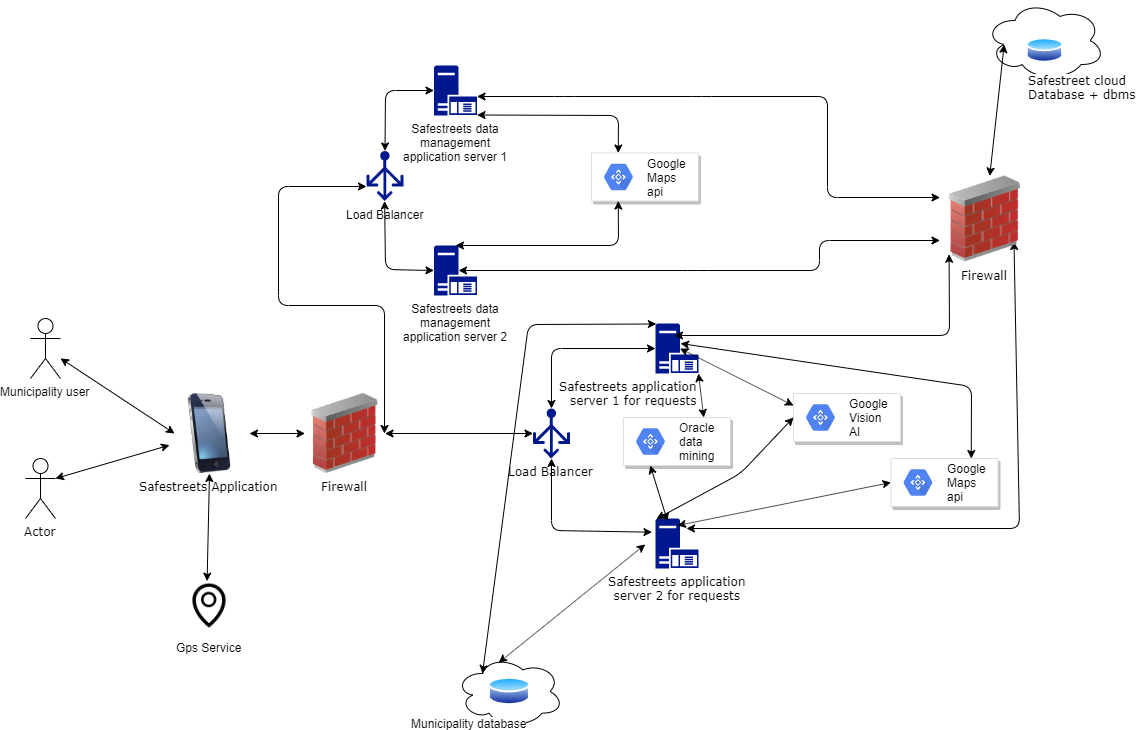
\includegraphics[scale=0.465]{Diagrams/overview.png}
	\caption{Architectural overview}
\end{figure}
\FloatBarrier
In the diagram above we can immediately distinguish 3 layers that make up the entire architecture. Servers manage the logic layer whereas databases manage the data layer and finally the client smartphone is where the presentation layer takes place. \\
The architecture has 2 clusters of application servers and two "types" of servers which deal with different tasks. One type of server handles the request by the user and the other one manages the reports by the private users and the authentication. Every cluster contains 2 servers of the same typology. Every server contained in one cluster access the system database whereas instead only the two servers dedicated to requests access the external one (which is the external database of the municipality). Servers which reside in different clusters don't communicate with each other to guarantee the service. Also servers of the same cluster don't communicate with each other. The workload balancing between servers of the same cluster is managed by to load balancers.\\
The client, in order to receive the service, will speak directly and only to the firewall placed at the entrance of the system. The first firewall (the one near the SafeStreets application in the diagram) is the element that will route the user messages to the right cluster based on the type of the request. In this case that firewall has not only a security function but it also behaves as a gateway which routes packets. All the clusters are placed inside the DMZ (between two firewalls) for security reasons. They must be accessible from the external network. The second firewall divides clusters from the system database. The database will have to be accessible only from the clusters for security reasons and because of this fact they are outside of the DMZ. \\

\begin{figure}[h]
\subsection{Component view}
Here there is a description of the software components that will be implemented in the specific hardware. The diagram is not horizontal in order to make it more readable. 
\\
	\includegraphics[scale=0.133, angle=-90]{Diagrams/Component diagram.png}
	\caption{Component diagram}
\end{figure}
\FloatBarrier

With this diagram our purpose is to show the internal software architecture of SafeStreets. \\
The main components are the user client application, the requests server application and the data management server application. The external interfaces are SafeStreets cloud database, the municipality database, the GPS interface, Google Maps, Oracle Data Mining API and Google Vision.\\
These main components contain smaller modular components that communicate with each other and with the external interfaces to complete different functions.\\
Now we will describe the internal components and the external interfaces in detail. \\

\paragraph{\textbf{User Client Application}}
The User Client Application is situated in the user's smartphone. It contains the Data Manager, the View and the Communication Manager:
\begin{itemize}
\item \textbf{Data Manager}\\
This component is responsible of taking the user's position in the world using the GPS service offered by his smartphone. Those data will be sent to the server in case he selects a service that uses the GPS localization. \\
\item \textbf{View}\\
This component is the view part of the MVC pattern. It takes data provided by the controller situated in the Server and shows them to the user with its interface.
\item \textbf{Communication Manager}\\
The Communication Manager is responsible for the network.
It manages all the communication from the client to the server and vice versa.\\
\end{itemize}

\paragraph{\textbf{Requests Server Application}}
This component is situated in the two servers of one of the Requests Server Application cluster and contains a Communication Manager, the User Requests component, the Municipality Suggestions Requests component and the Data Mining one:
\begin{itemize}
\item \textbf{Communication Manager}\\
It has the same function of the one situated on the client. It dispatches and receives message from the client application.
\item \textbf{User Requests}\\
This component manages all the requests coming from the private users and the municipality, except for the suggestions requests. It contains a User Requests Manager, that elaborates the requests and asks for the necessary data to the Data Storage Manager. The User Requests component contains also the Data Storage Manager that retrieves the requested data querying the SafeStreets external database.
\item \textbf{Municipality Suggestions Requests}\\
This component deals with the suggestions requests made by the municipality. It contains the Municipality Suggestions Requests Manager that receives the requests from the Communication Manager and asks for the needed data to the Data Mining component. When the suggestion is ready, the Data Mining component send it back to the Municipality Suggestions Request component, especially to the Municipality Suggestions Requests Manager, that dispatches it to the Communication Manager that sends it to the Client Application.


\item \textbf{Data Mining}\\
This component is responsible for the retrieval of the information needed to provide suggestions to the municipality. It receives from the Municipality Suggestions Requests Component a request for suggestions. It contains the Data Requests Manager that handle the received request and asks for data to other two components, also situated in the Data Mining Component. They are the Data Storage Manager that provides the data about the violation and the streets that SafeStreets has in its cloud database, and the other is the Municipality Data Storage Manager that provides the data, again about the violations and the streets, but now querying the Municipality external database. When all those data arrive to the Data Requests Manager, it dispatches them to the Suggestions Creation Manager, that runs a data mining algorithm provided by an Oracle API in order to merge the received data and retrieve information useful to provide suggestions to the Municipality. Finally the result is sent back to the Data Requests Manager, that sends it to the Municipality Suggestions Requests Component. 
\end{itemize}

\paragraph{Data Management Server Application}
This component is situated on the two server of the Data Management Server Application cluster. It contains the Communication Manager, Reports Component and the Authentication one:
\begin{itemize}

\item \textbf{Communication Manager}\\
It has the same function than the one situated in the Requests Server Application.

\item \textbf{Reports}\\
This component is responsible for the violation reports. It receives the reports from the Communication Manager and it contains a Report Validity Manager that checks that the violation data inserted by the user are correct. Then it has the Photo Analysis Manager that retrieves the license plate of the violator from the photograph using an algorithm provided by an external API (Google Vision) that scans the photo. Finally there is a Data Storage Manager that takes all the information about the violation (license plate, type of violation, description, position, date and hour) and stores them in the SafeStreets database.

\item \textbf{Authentication}\\
The Authentication component manages all the operation about login, sign up and logout.
It contains a Credentials Validity Manager that checks the user's input (both in login and sign up) and checks if he is logged in whenever he wants to logout. Then it contains also a Data Storage Manager that queries the SafeStreets Cloud Database in order to receive the account data that has to be checked by the Credential Validity Manager and stores the user's account data in the database in case of sign up.
\end{itemize}

\paragraph{\textbf{External Interfaces}}
Some of the components already described have to communicate with external interfaces in order to guarantee specific functionalities. These interfaces are:
\begin{itemize}
\item \textbf{SafeStreets cloud database}\\
This component is shared with both Servers. In each of the two servers there is a component that is the only one that communicates with this database and it's the Data Storage Manager, that can both query to retrieve data and add new information into the database.
\item \textbf{Municipality Database}\\
This component communicates with the Requests Server Application, in particular with the Municipality Data Storage Manager, that can only query to obtain information in order to create suggestions for the Municipality. This database is in read-only mode.
\item \textbf{GPS}\\
This external component is necessary for the user's automatic localization. It communicates with the User Client Application, in particular with the Data Manager that is the one specialized in retrieving the position information (city and street) from the GPS service offered by the user's smartphone.
\end{itemize}




\begin{figure}[h]
	\subsection{Deployment view}
	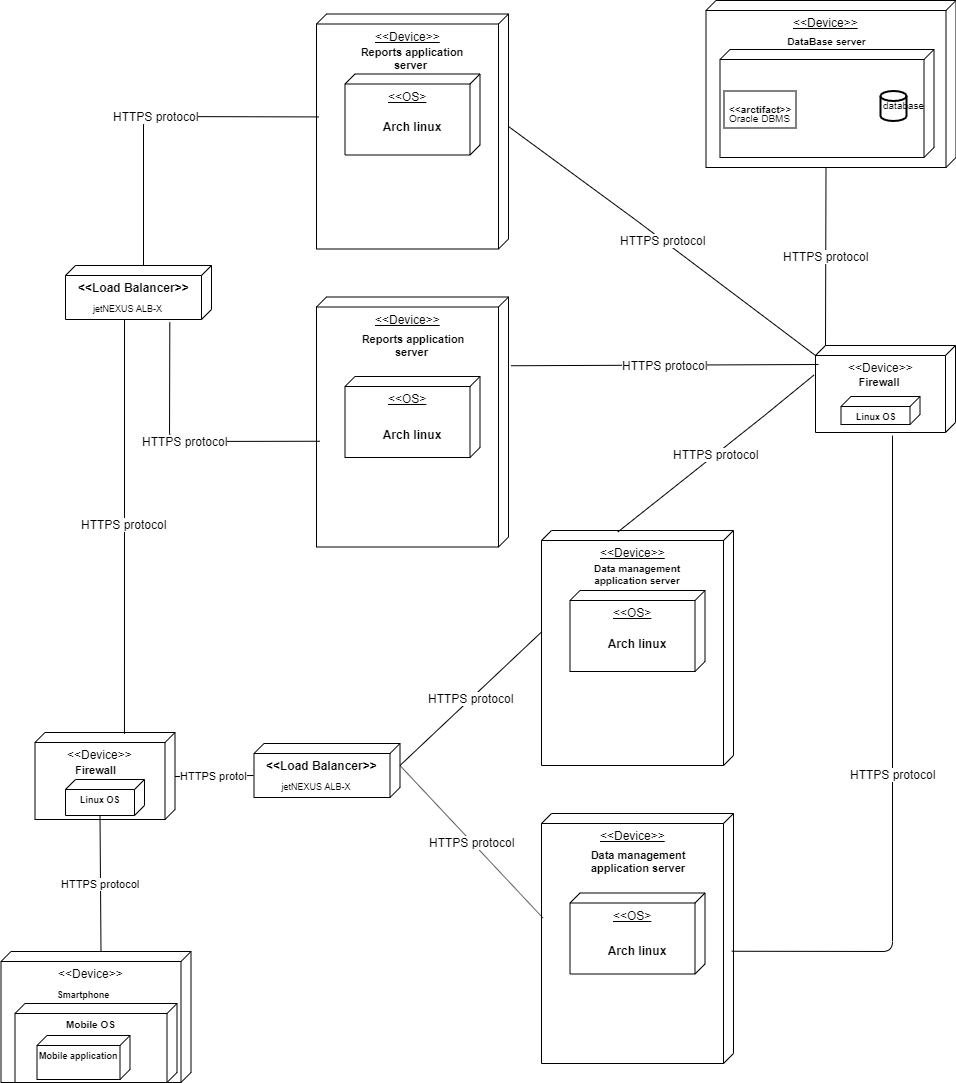
\includegraphics[scale=0.465]{Diagrams/Deployment diagram.png}
	\caption{Deployment diagram}
\end{figure}
\FloatBarrier

This diagram is very similar to the one in the overview. It expresses some aspects which have been already explained and some others explained only here. In fact we can see all the operating systems for each server and also the protocol used in the communication between the devices.
Here you can find a brief description of what the single components do:
\begin{itemize}
\item \textbf{Firewall:} Firewalls are well known for sure by the majority of the people but we think that it is important to describe their operation the same. Firewalls are placed between the internal network and the external ones.They are used to filter the incoming/outgoing packet traffic. Through a set of rules they decide if a packet can pass or be blocked.  This can be very useful to guarantee a better system security.
\item \textbf{Load Balancer:} Load Balancers are used to improve the workloads across multiple computing resources. Thanks to the load balancer the load can be balanced in an optimal way.This can make the system more performing and can also improve the fault tolerance of the system because of redundancy.
\item \textbf{Servers:} In this architecture we can find two clusters, each one containing 2 application servers. The clusters are specialized with no overlap of functionalities. One is specialized in the managing of the reports by the private users and authentication. It must update the database with the new incoming data only after having done all the checks about the validity and correctness of the report.\\
In case of authentication, this cluster is responsible to manage all the requests of login, sign up and logout and it communicates with the system database in order to retrieve credentials and insert new accounts data.\\
The other server deals with the management of the requests by the private users or municipalities. It is in charge of checking the correctness and validity of the request. In case of a suggestions request by the municipality, the system merges the data from the Safestreets and the Municipality databases with the help of a Data Mining external API provided by Oracle in order to provide the suggestion to the municipality user.\\
For all the other types of requests, the system takes the necessary information from the Safestreets database in order to send them to the user.\\
\item \textbf{Databases:} They are cloud databases managed thanks to an API that will be given by the provider of the service. We have only one cloud database used to store all the Safestreets data. Another cloud database is the external one of the municipality. Safestreets has only a special view of the part of the municipality database concerning the accidents. All these cloud databases use SQL.
\end{itemize}
\newpage
\subsection{Runtime View\\}
\paragraph{Sign Up Runtime View\\ \\}
With this sequence diagram we explain which components come into play and how they interact when a user signs up.
This process is the same both for private users and municipality.\\
When the user pushes the sign-up button, the View sends the sign up request to the Client Communication Manager that provides to dispatch it, together with the user's submitted personal data, to the Server Communication Manager, through the use of the Load Balancer in order to manage the load and assign it to one of our two servers. Then the Server Communication Manager is responsible to send all the data to the Credentials Validity Manager that checks the validity of the inserted data, controlling if the password complies our restrictions. Then it sends to the Data Storage Manager a request to query the SafeStreets Cloud Database to discover if there is already or not an existing account associated with the username inserted by the user. After having received a response from the Database, the Data Storage Manager sends the response to the Credentials Validity Manager that checks it. In case there is already an existing account, the Credentials Validity Manager sends an error message to the Server Communication Manager that propagates it to the Load Balancer and then to the Client Communication Manager informing it about a malformed request or an already-in-use account. The Communication Manager sends the message to the View that shows it to the user. \\
In case all the verifications are ok, the Credentials Validity Manager sends the account data to the Data Storage Manager, that cares about inserting it in the database. After having received the feedback from the database, the Data Storage Manager sends it to the Credentials Validity Manager that checks it. If the confirmation isn't valid the Credentials Validity Manager propagates a message error that, with the usual path, is received by the user. If the confirmation is ok the Credentials Validity Manager uses the same procedure to send to the user the confirmation message.

\begin{figure}[h]
	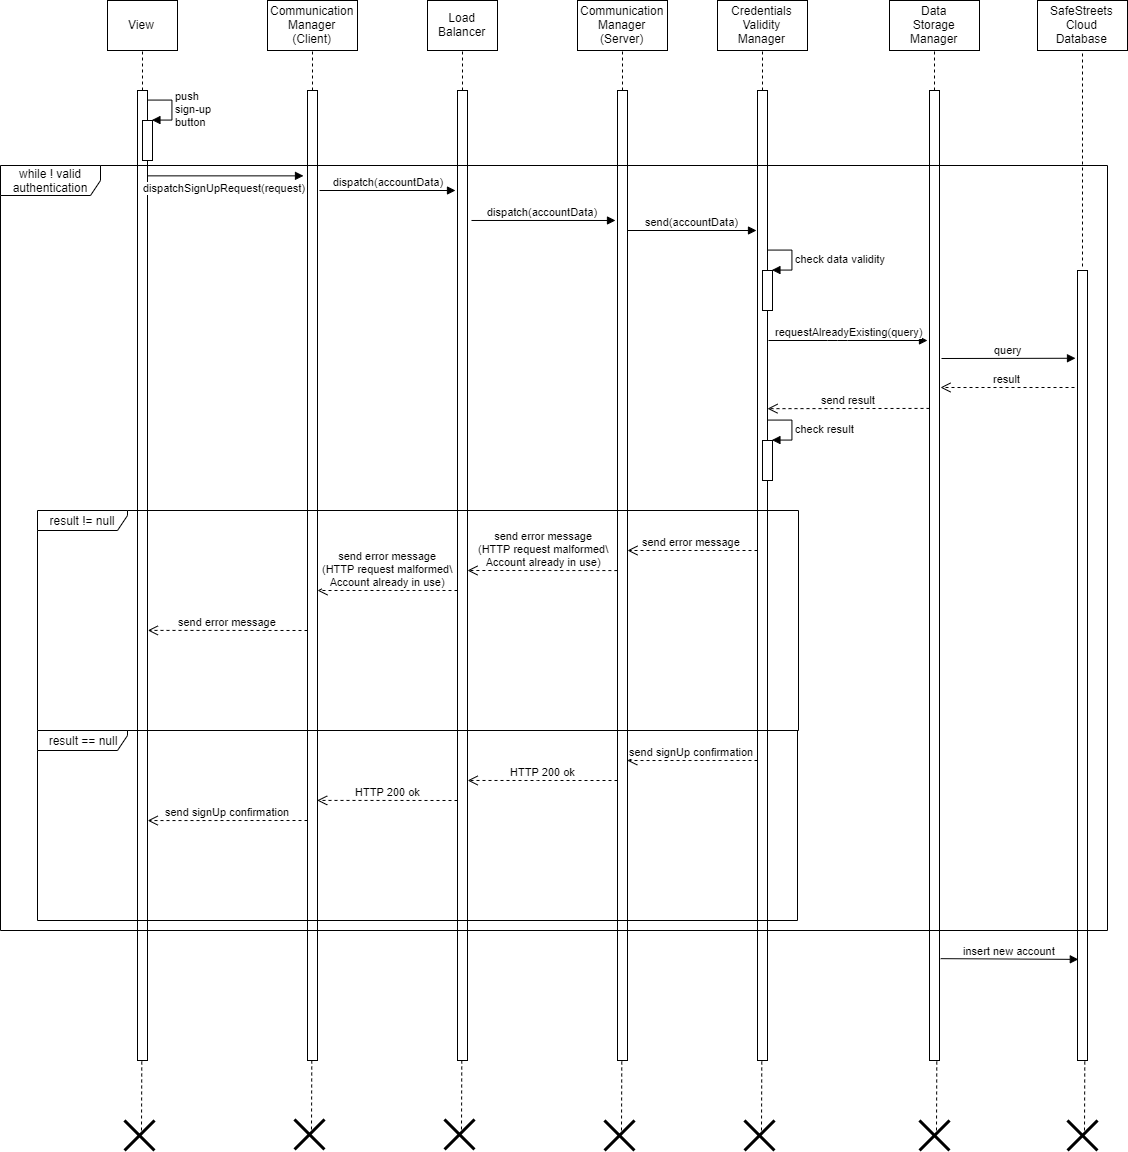
\includegraphics[scale=0.39]{Diagrams/Sequence Diagrams/Runtime View Diagram signup.png}
	\caption{Sign Up Sequence Diagram}
\end{figure}
\FloatBarrier

\paragraph{Login Runtime View \\ \\}

In this sequence diagram we explain which are the components involved and how they communicate with each other. \\
When the user pushes the login button, the view propagates the login request to the Client Communication Manager that is responsible to dispatch it to the Server Communication Manager, also thanks to the use of the Load Balancer that has the same function explained for the signing up. \\
Then the Server Communication Manager sends the request with the credentials to the Credentials Validity Manager, that elaborates a query to check if the credentials submitted by the user match an existing account in the database. The query is sent to the Data Storage Manager that dispatches it to the SafeStreets Cloud Database. When the Data Storage Manager receives an answer from the database, it sends the result to the Credentials Validity Manager that checks if it's valid or null. \\
If it's null it dispatches an error message to the Server Communication Manager that sends it to the client (through the Load Balancer) as a HTTP malformed request or wrong credentials. Finally, when the Client Communication Manager receives the error message, it sends it to the View that displays it to the user.\\
If the result is not null, the Credential Validity Manager sends the login confirmation message to the Server Communication Manager, that cares about sending it to the user in the usual way.

\begin{figure}[h]
	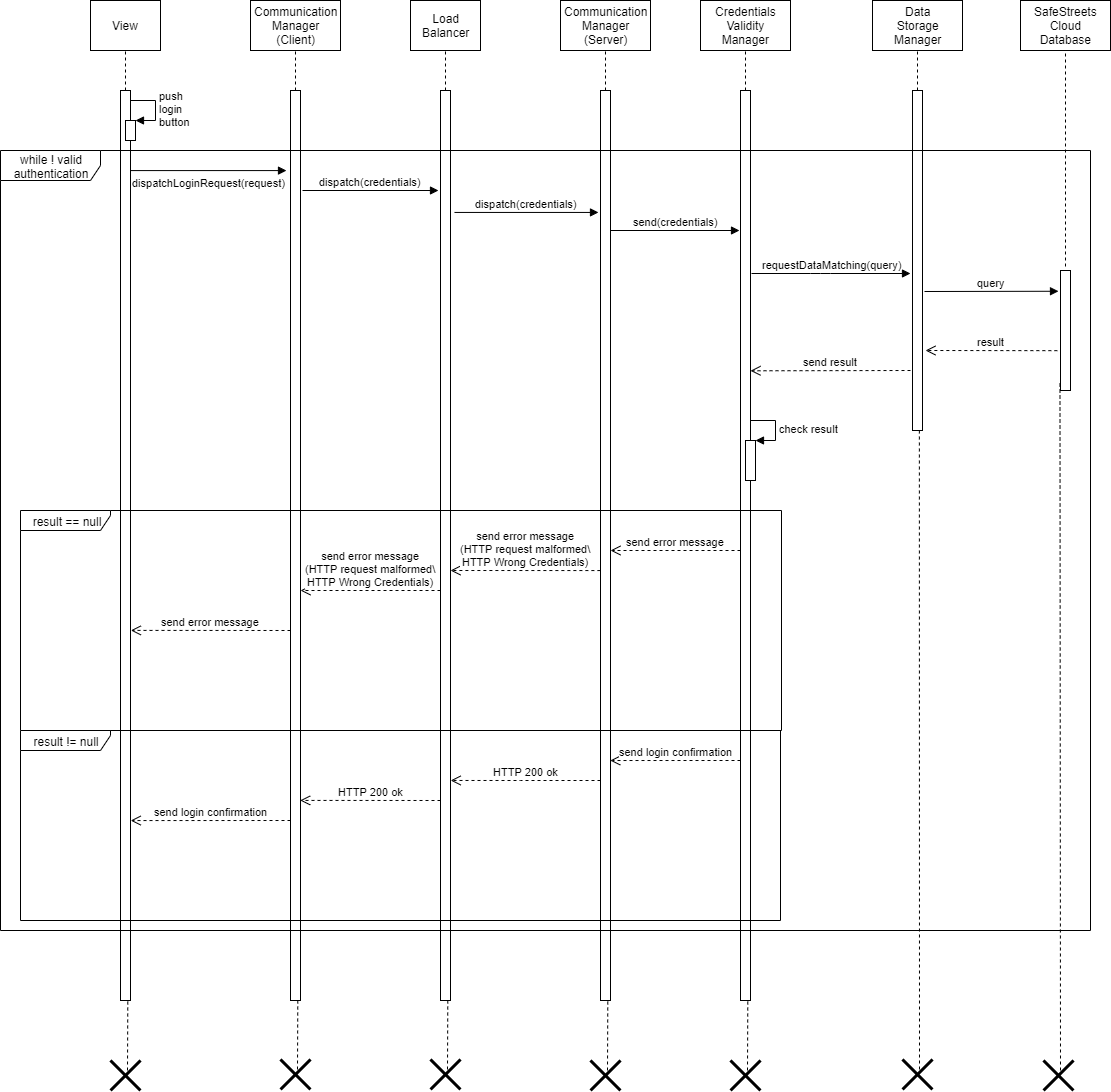
\includegraphics[scale=0.42]{Diagrams/Sequence Diagrams/Runtime View Diagram login.png}
	\caption{Login Sequence Diagram}
\end{figure}
\FloatBarrier


\paragraph{Report Runtime View \\ \\}

In this sequence diagram we explain the process of a Violation Report. \\
When the user submits all the violation information by pushing the report button, the View sends the report to the Client Communication Manager. It dispatches the report to the Load Balancer that sends it to the Server Communication Manager. It sends the report to the Report Validity Manager that sends the city and the streets to Google Maps in order to check if they exist. Then it checks the correctness of the report. To do this it checks if the violation type belongs to one of the categories suggested by the municipality.
After that, if the report isn't correct it sends back to the Server Communication Manager an error message. The Server Communication Manager will propagate it to the client (through the Load Balancer) as invalid input.
Then, the Client Communication Manager sends the error message to the View, that shows it to the user, that can reformulate the report and redo the same process in order to do a new submission. \\
If the report is correct, the Report Validity Manager sends the confirmation back to the Server Communication Manager that, with the same process of the error communication, dispatches it to the client as HTTP 200 OK in order to finally make the View display the confirmation to the user. \\
In the meanwhile the Report Validity Manager sends to the Photo Analysis Manager the photo appended to the report. Then the photo is sent to Google Vision that analyses it in order to retrieve the license plate. Then the Photo Analysis Manager receives the plate found by Google Vision and dispatches it to the Report Validity Manager. \\
It send all the data about the report to the Data Storage Manager that provides to insert it in the SafeStreets Cloud Database that sends back a confirmation.
The Data Storage Manager checks the response. If the data has not been inserted into the database, the Data Storage Manager sends an error message to the Server Communication Manager that propagates it to the user in the usual way. Otherwise, if the data has been correctly inserted into the database, the Data Storage Manager sends the confirmation to the Server Communication Manager that cares about propagating it to the user.


\begin{figure}[h]
	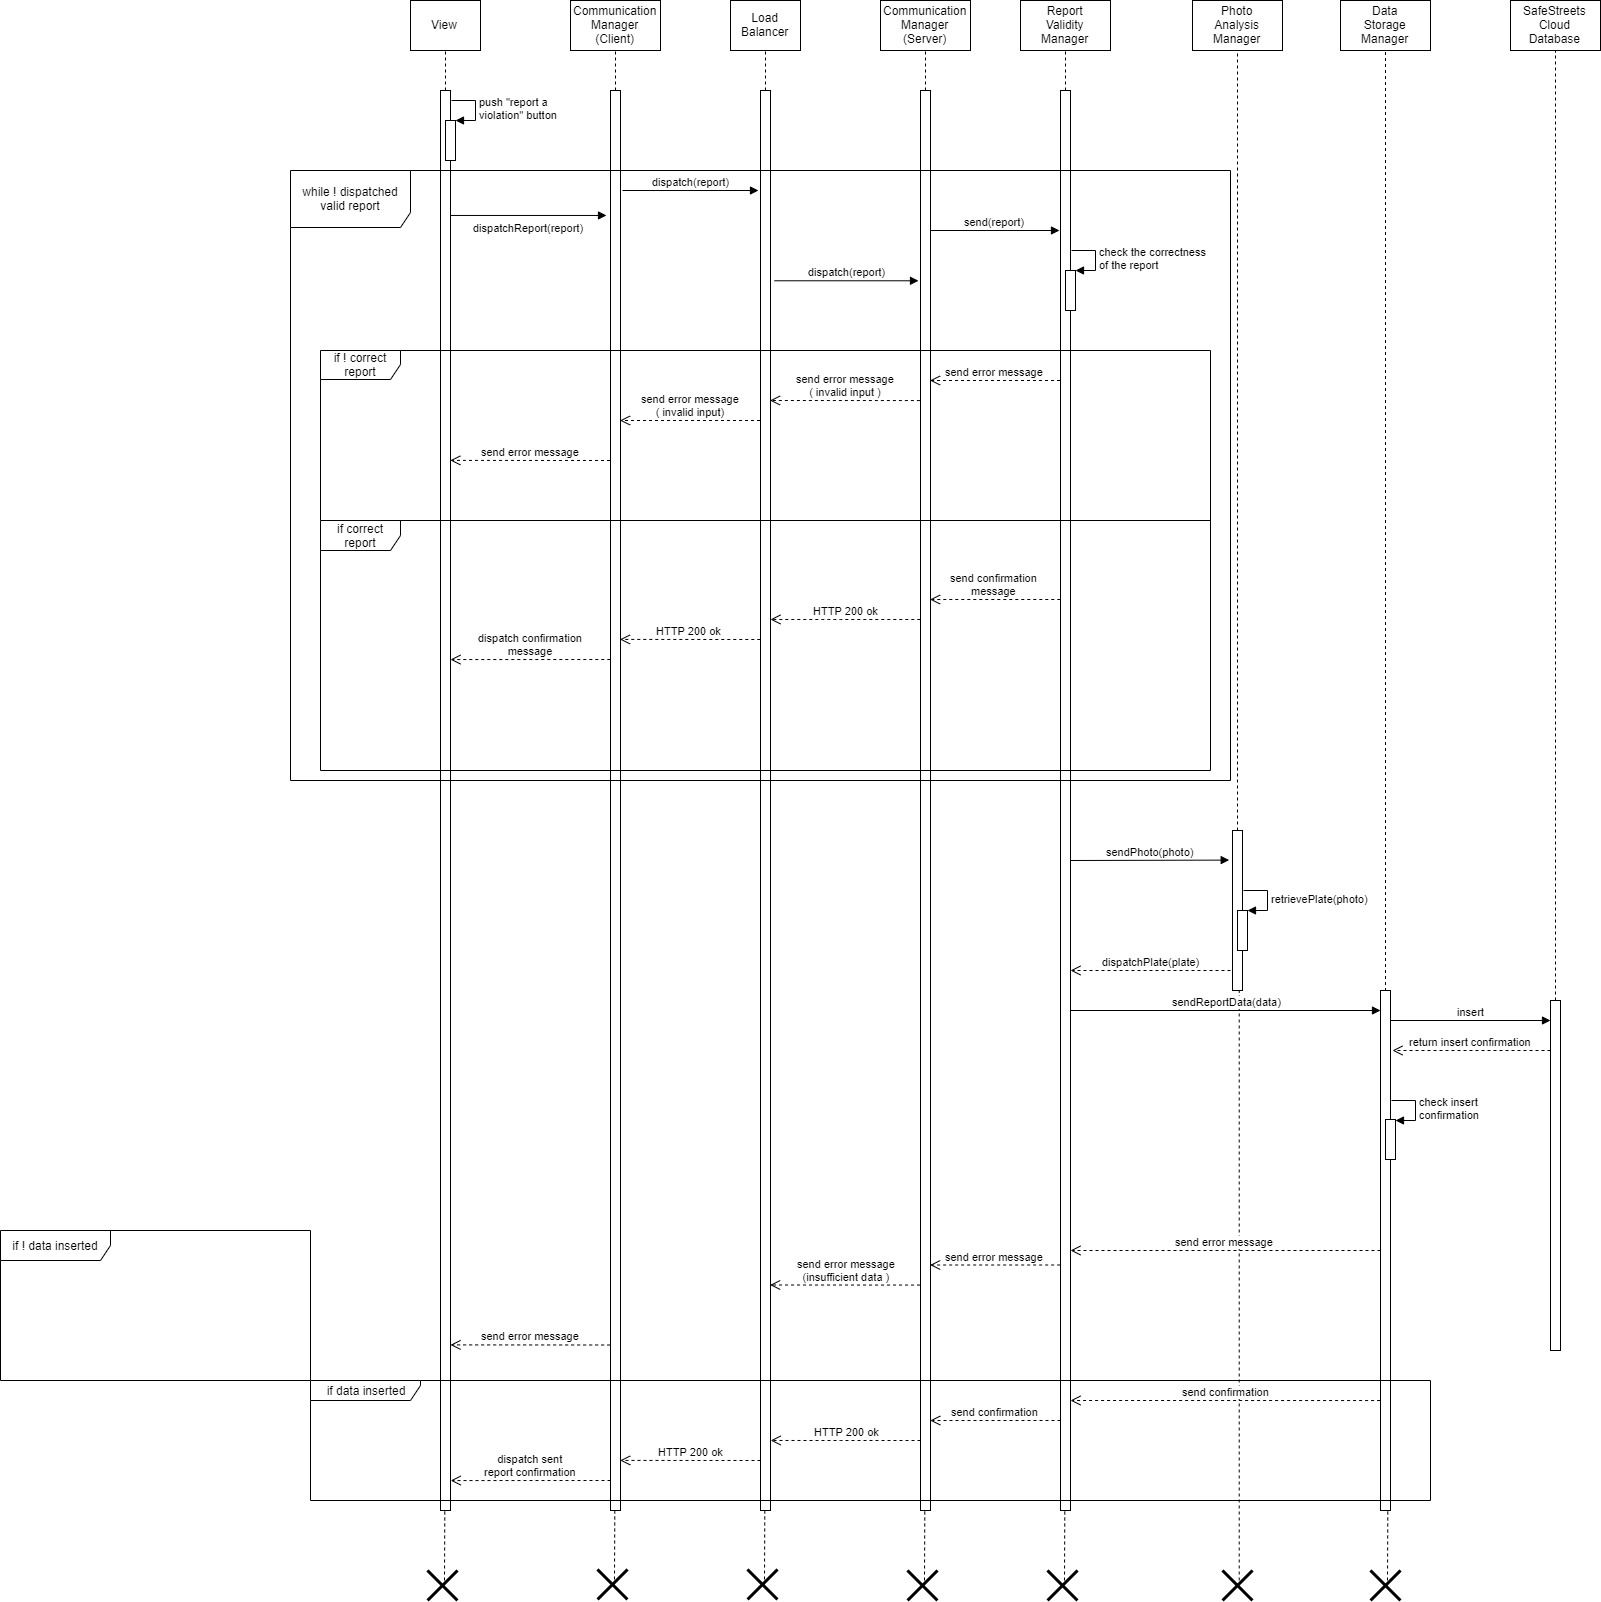
\includegraphics[scale=0.298]{Diagrams/Sequence Diagrams/Runtime View Diagram report.png}
	\caption{Report Sequence Diagram}
\end{figure}
\FloatBarrier

\paragraph{User Request Runtime View\\ \\}

With this sequence diagram we show how the process for user requests is structured.
This process is the same both for private users and municipality and this process is the same for all the types of requests except the municipality's request for suggestions.\\
When the user submits a request, the View dispatches it to the Client Communication Manager that cares about sending it to the Server Communication Manager (through the Load Balancer). Then the request is sent to the User Request Manager that sends the city and the street found on the request to ask Google Maps if there is an existing city and street. \\
After having received a response, the User Request Manager checks it and if the place inserted by the user doesn't exist it provides to send an error message to the Server Communication Manager, that sends it to the Load Balancer and then to the Client Communication Manager as HTTP Malformed Request. Then the Client Communication Manager dispatches it to the View that shows it to the user.\\
Otherwise, if the request is valid, the User Request Manager sends a data request to the Data Storage Manager, that queries the SafeStreets Cloud Database in order to receive the necessary information. After having received the result, the Data Storage Manager dispatches it to the User Request Manager that checks it. \\
If the database has sent a null result, the User Request Manager sends an error message to the Server Communication Manager that cares about sending it to the Client Communication Manager (through the Load Balancer).
Then the message is sent to the View that displays it to the user.
If the database returns a not null result, the User Request Manager sends the requested data to the Server Communication Manager that, in the usual way, dispatches it to the Client Communication Manager, that sends it to the View. Finally the View displays the information to the user.


\begin{figure}[h]
	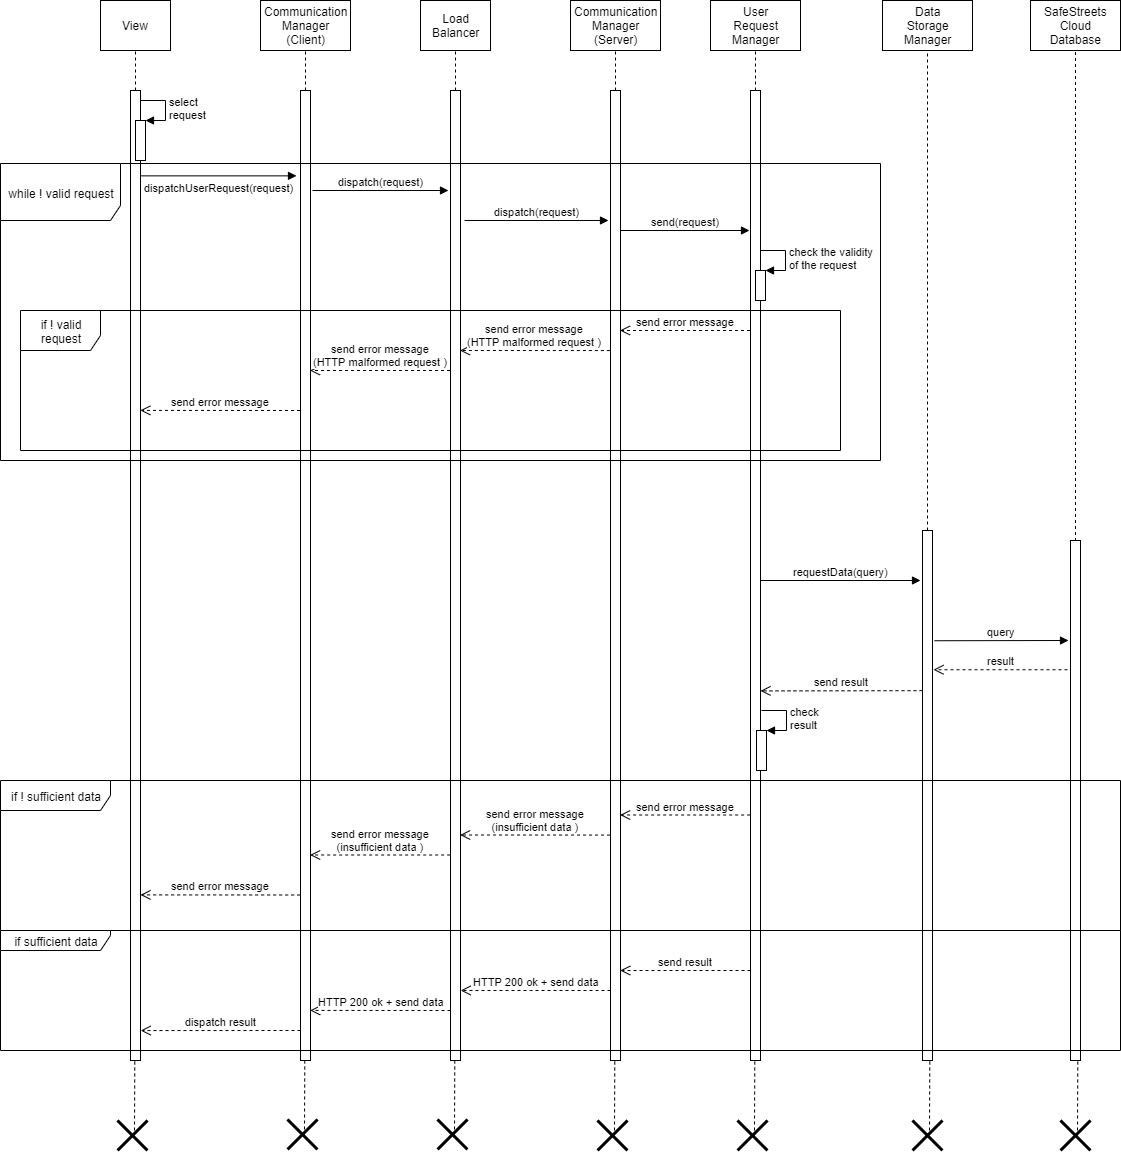
\includegraphics[scale=0.387]{Diagrams/Sequence Diagrams/Runtime View Diagram user request.png}
	\caption{User Request Sequence Diagram}
\end{figure}
\FloatBarrier


\paragraph{Municipality Suggestions Request Runtime View\\}

This sequence diagram explains the process with which the municipality requests and receives suggestion to make the streets safer. \\
When the municipality user submits the request for suggestions, the View shall forward it to the Client Communication Manager. It dispatches the request to the Load Balancer that sends it to the Server Communication Manager. It sends the request to the Municipality Suggestions Request Manager, that searches through Google Maps if the user has inserted an existing city. After having received a response, the Municipality Suggestions Request Manager checks it and checks also if the city matches with the Municipality. If the city doesn't exist or isn't correct, The Municipality Suggestions Request Manager sends an error message to the Server Communication Manager, that propagates it to the user in the usual way.\\
If the city is correct the Municipality Suggestions Request Manager asks the Data Request Manager for the necessary data. it sends a request to the Data Storage Manager, that queries the SafeStreets Cloud Database. After having received a result from the Database, the Data Storage Manager sends it to the Data Request Manager. It does the same procedure for the Municipality data, making a request and sending it to the Municipality Data Storage Manager that queries the Municipality Database.\\
After having collected all the information, the Data Request Manager sends the data to the Suggestions Creation Manager, that cares about sending it to the External Data Mining API offered by Oracle. It is responsible for merging all the information and creating suggestion from the result, through the use of a data mining algorithm. \\
After that it returns the suggestions to the Suggestions Creation Manager that dispatches them to the Result Handler. This component sends the created suggestions to the Server Communication Manager that, in the usual way, cares about sending the data to the View, that will display it to the Municipality User.
\newpage



\begin{figure}[h]
	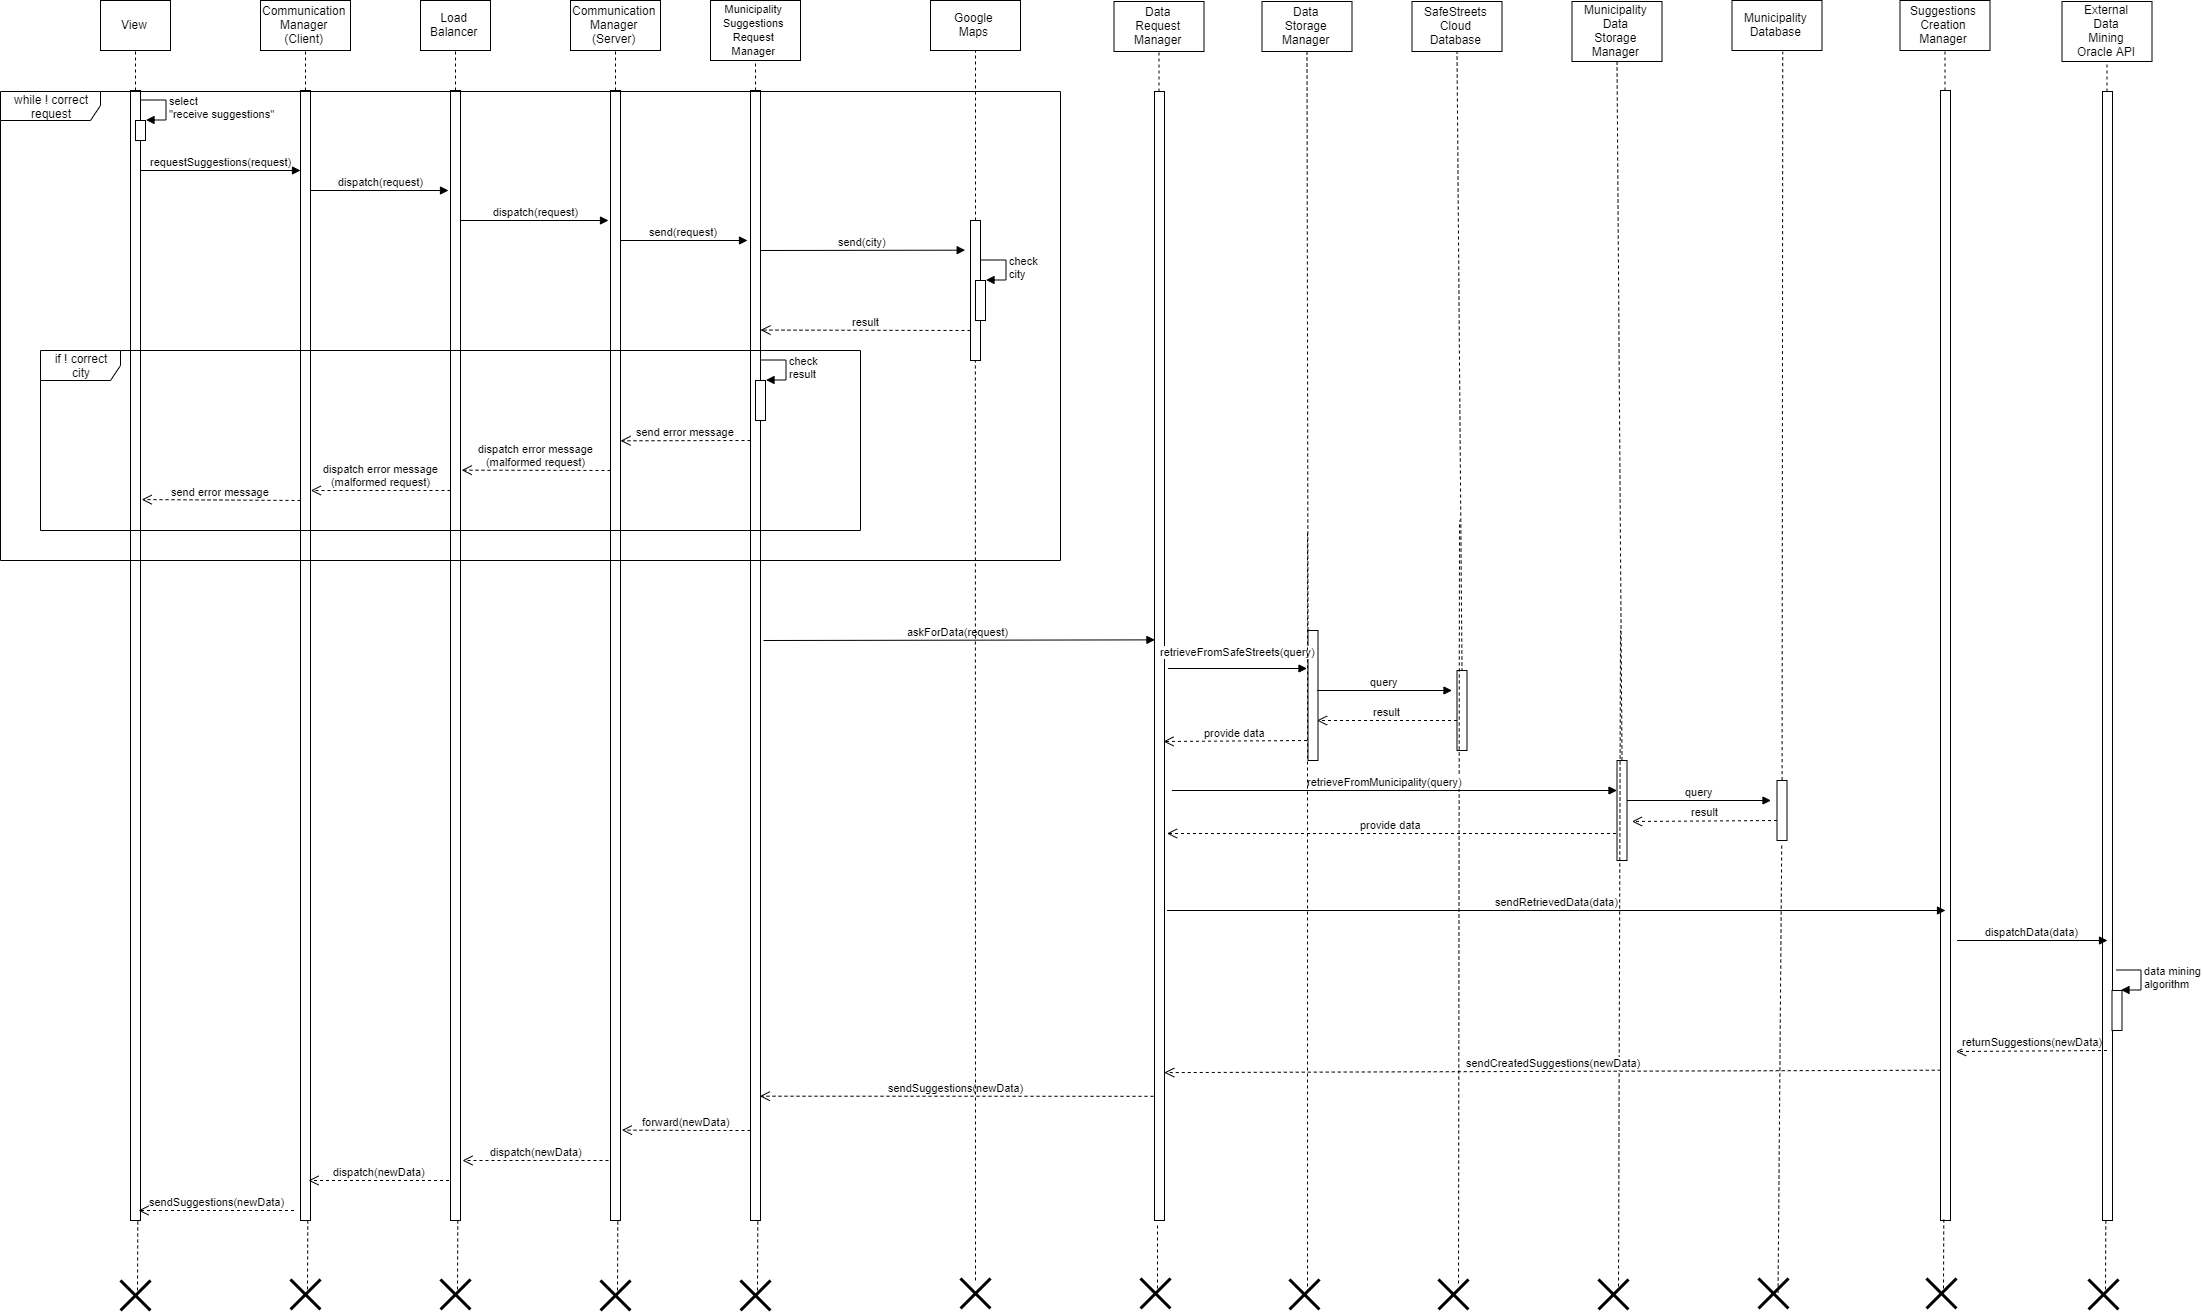
\includegraphics[scale=0.206]{Diagrams/Sequence Diagrams/Runtime View Diagram suggestions.png}
	\caption{Municipality Suggestions Request Sequence Diagram}
\end{figure}
\FloatBarrier
\newpage



\subsection{Component interfaces}

This diagram is useful to understand which are the methods that the components use and how the components interact with each other. The diagram is made up in order to be consistent with the component diagram, that must have the same structure, and the sequence diagrams in the runtime view, that must have the same methods.\\


\begin{figure}[h]
	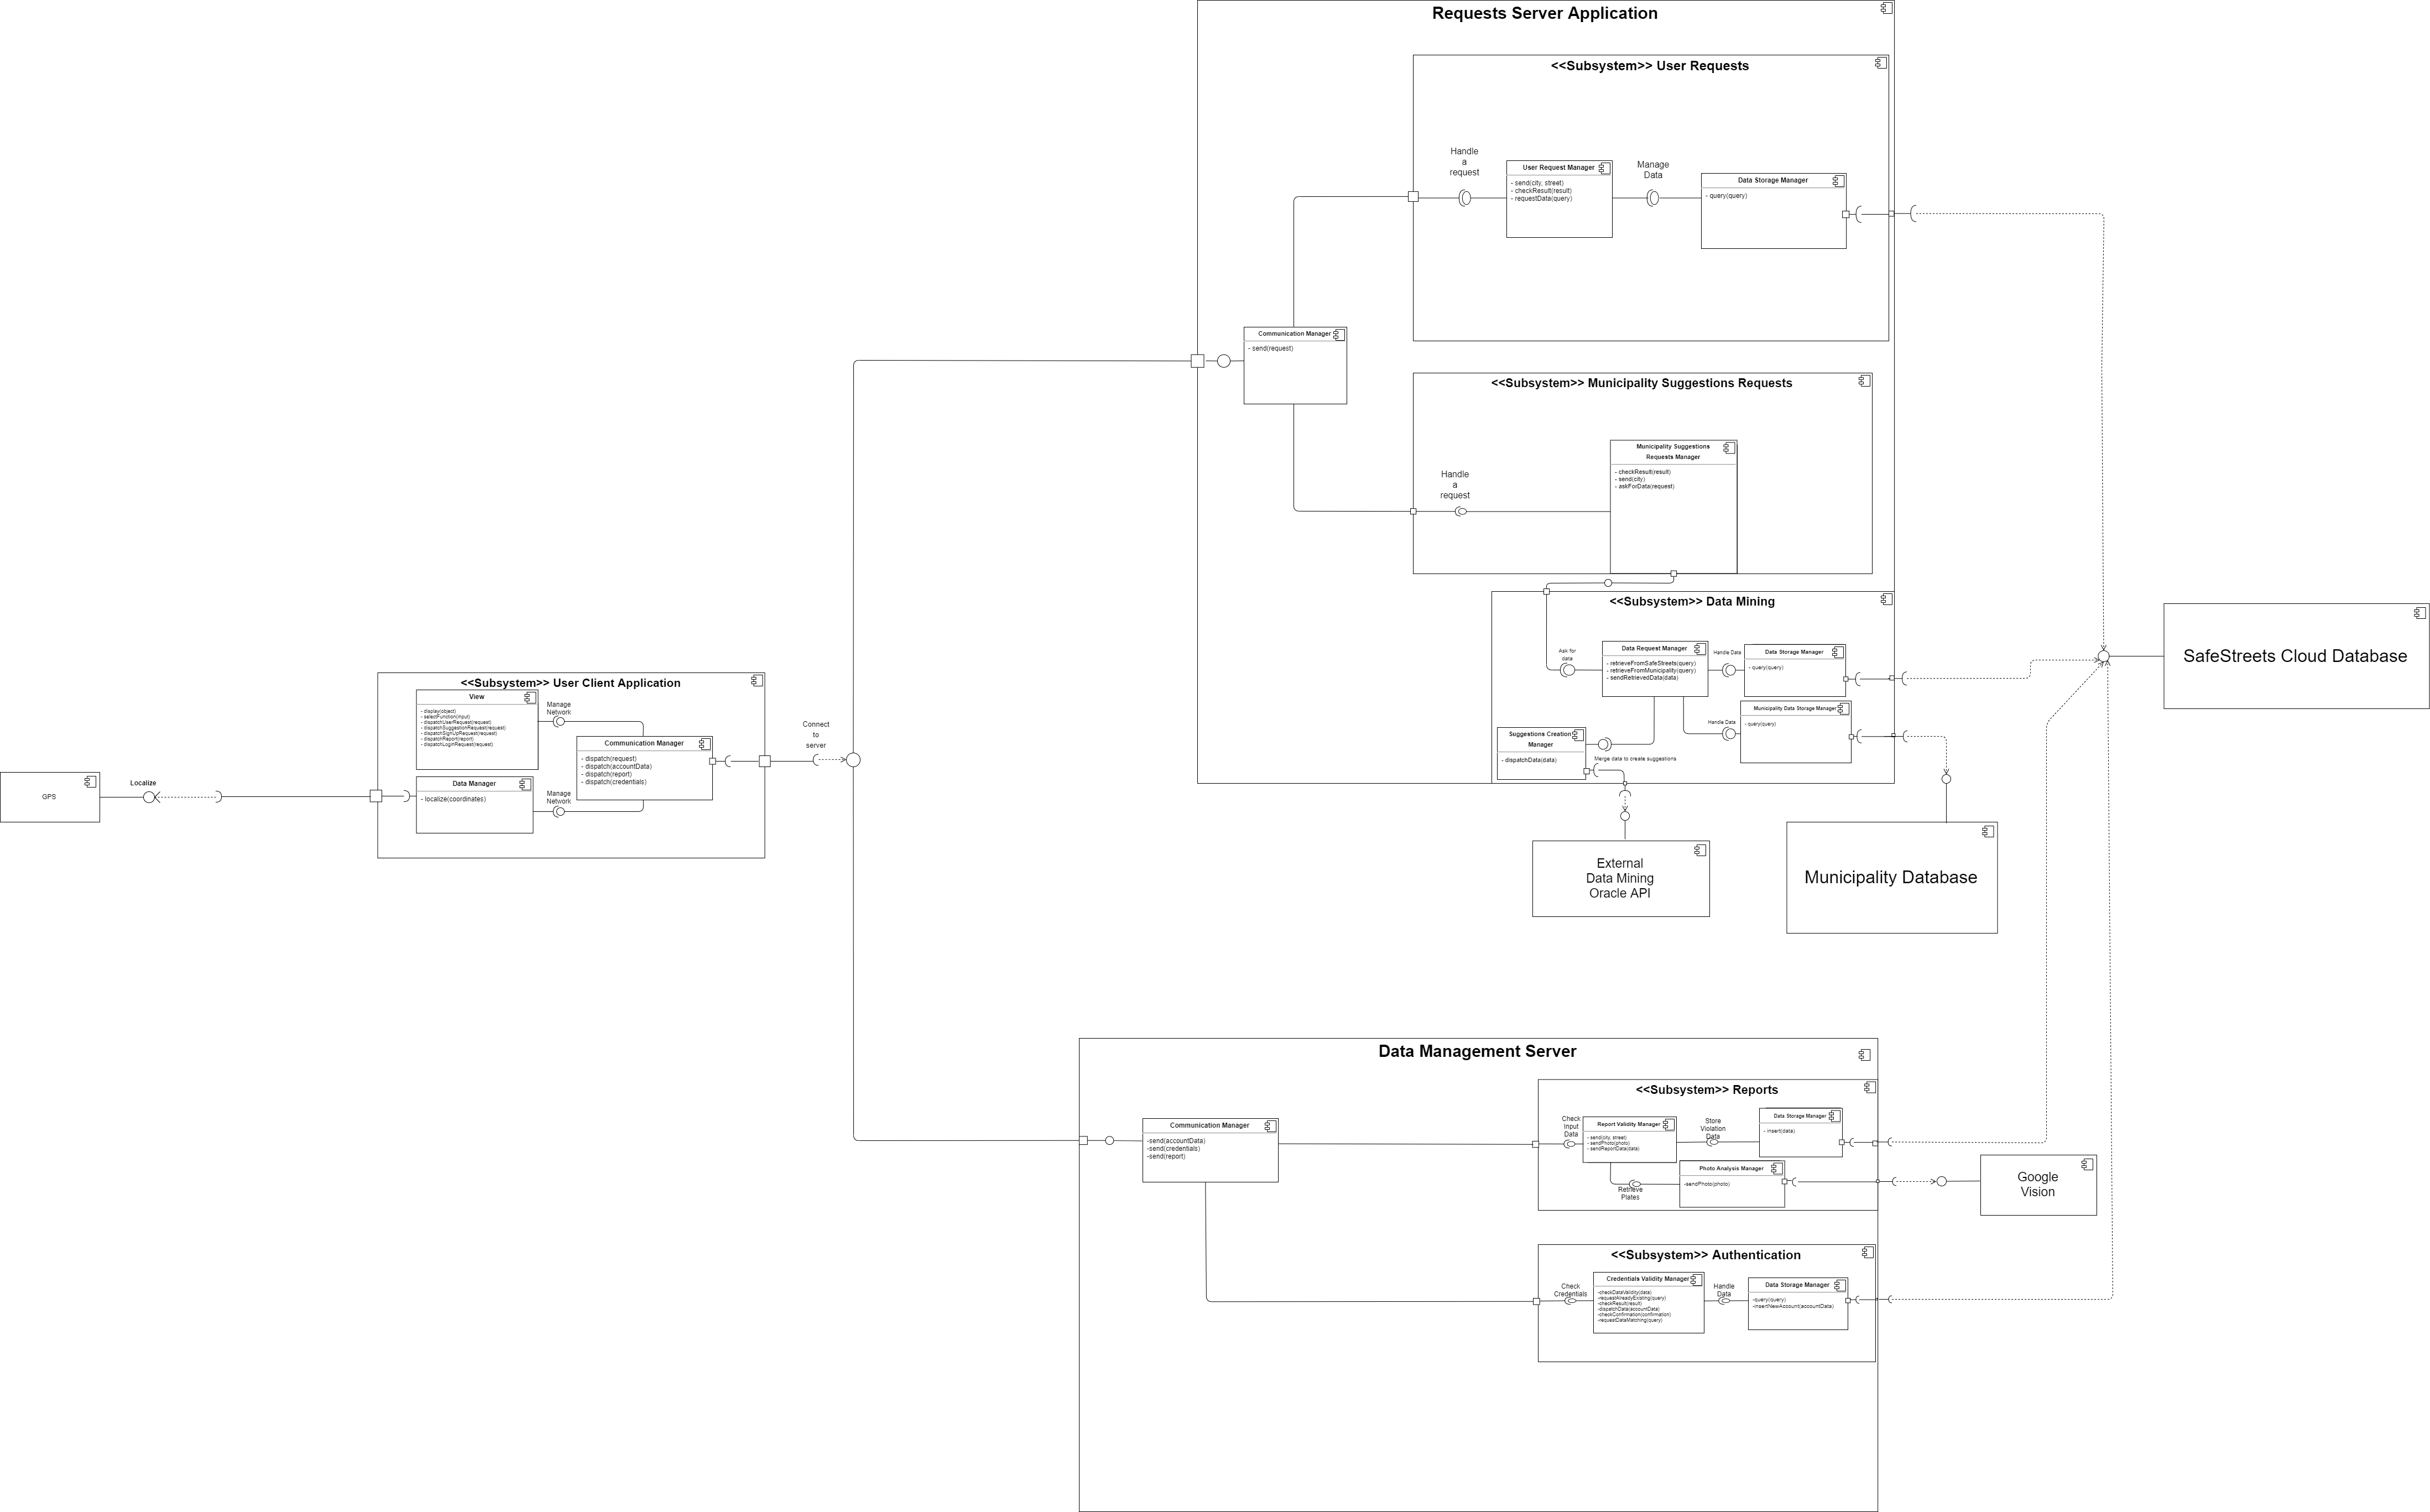
\includegraphics[scale=0.108]{Diagrams/Component Interface Diagram.png}
	\caption{Component Interface Diagram}
\end{figure}
\FloatBarrier

\subsection{Selected architectural styles and patterns}
We have selected an 4 tiers architecture. The entire system is a client-server application. The smartphone of the user implements only the presentation layer. This decision is due to the fact that we want the mobile application to be lightweight. We want the app to perform discreetly even with non-modern hardware phones. We want an application that limits as little as possible the hardware in a phone in terms of performance. The system data are stored in a database  whereas the systems uses also another database which is the one of the municipality.
The application logic is divided in two specialized clusters of application servers as already explained. We have chosen this to make the two interactions with the user (a user request or a user report) independent as much as possible.\\
 The data layer is implemented in the databases of the system.\\
The decision of having different layers is to make the system as maintainable as possible. Every layer will offer only a simple interface to receive data and another one to send data to another layer and nothing more. In this way the implementation details are hidden. This means that when the system is modified it cannot happen that the modification of a layer causes a chain of successive modifications in other layers caused by the latter.\\ \\
The system can be seen also as an example of MVC pattern:
\begin{itemize}
	 \item \textbf{Model:} The model is the component which store all the application data and check their integrity and so eventually modify the data structures to keep it. It is implemented in the databases (both the external and the internal one)
	 \item \textbf{View:} The view is the software component that deals with the presentation layer. It only show data and information to the user. This component is implemented in the user device (as already explained before)
	 \item \textbf{Controller:} The controller is the software component that contains and manages the application logic. In this system this logic layer must be implemented in the application servers. \\
In our case, in particular, it is divided in two subcomponents implemented in different devices. One part concerns the managing of the requests and the other one concerns with the reports of the user. The first its implemented in the servers for the request and the latter in the servers for the reports.
\end{itemize}
\subsection{Other design decisions}
Here it is possible to find another design decision which are not about patterns and design styles which are the following:
\begin{itemize}
	\item \textbf{ Use of cloud databases:} We have chosen cloud databases to store the systems data because in this way it is possible to decrease or increase the resources according to the load of requests or reports. In this way it is possible to balance the storage space according to the load automatically. A solution based on proprietary databases would have been probably more efficient in terms of performances but surely more critical in terms of allocation or deallocation of resources. Furthermore, another important aspect of this choice is the fact that the physical maintenance of cloud database is entrusted to third parties (the owners of the physical devices which are the providers of the cloud service).
	\item \textbf{Use of clusters:} The use of clusters has been decide in order to try to make the system possibly more performing but above all, more fault tolerate. We have discarded the idea of having a single server instead of a cluster precisely because of this aspect. If the single server is down, then, the entire service will surely be inaccessible for the user. \\
The use of clusters is excellent as it makes the system more scalable. In fact, it is also easy to add additional servers possibly in the future.
	\item \textbf{Use of load balancers:} The use of load balancers has been decided to make the system more performing. In fact the throughput can be maximized and the response time minimized considerably. 
	\item \textbf{Use of relational databases:} For this system we have chosen relational databases. On of the reason about this decision is the fact that the data that the system manages and stores is well defined and structured. We know that sometimes operations like "join" between different tables can affect the system and makes it slower. However, we think that this aspect will not cause relevant problems in our system. In fact the performance constraints are large enough to not cause problems in our opinion. Furthermore, relational databases have been used for several years and they are used also nowadays for a lot of applications. Because of this, we have a strong theoretical background about them. This is not always true for not relational databases.
	
\end{itemize}

\begin{figure}[h]
	\section{User interface design}
Here there will be shown the user interfaces with the help of UX diagrams. In particular there is shown the flow that the user will follow to navigate inside the application. Some aspects concerning the user interfaces design have been already treated in the "Requirement Analysis and Specification Document",if the reader wants to understand in a better and more detailed way, he/she is strongly suggested to refer also to it. In this document it is described only the flow that the user must follow to use the application.
UX diagrams:\\
	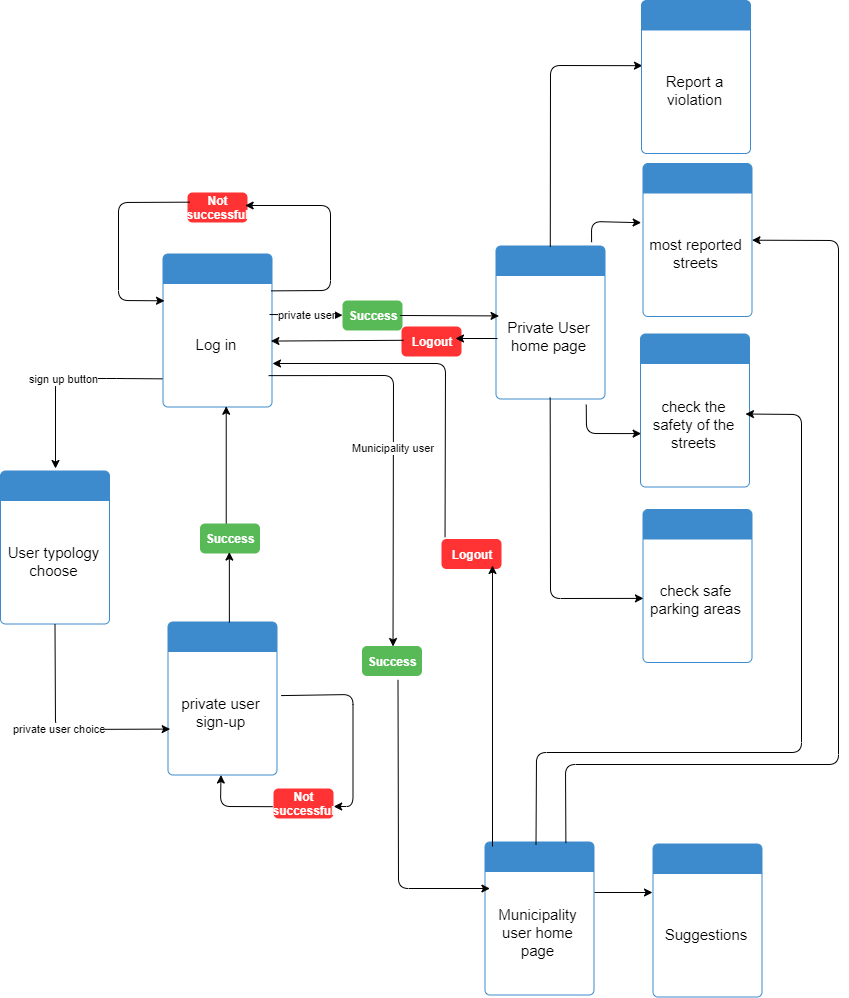
\includegraphics[scale=0.48]{Diagrams/UX diagram.png}
	\caption{UX diagram}
\end{figure}
\FloatBarrier
\section{ Requirements Traceability}
Here it is possible to find an explanation about how the requirements in the rasd map to the to the design elements that can be found in this document.

\begin{longtable}{| p{7 cm} | p{8 cm} |} \hline
		Component  & Requirements (RASD) 
		 \\ \hline
		\newline \textbf {View} &
		\begin{itemize}
		\item \textbf{$[R1]:$:}The system must allow the user to take a picture. 
		\item \textbf{$[R2]:$}The system must allow the user to indicate the street where the violation occurred. 
		\item \textbf{$[R3]:$}The system must allow the user to indicate the hour and the date when the violation occurred. 
		\item \textbf{$[R4]:$}The system must allow the user to insert a brief description of the violation. 
		\item \textbf{$[R5]:$} The system can localize his/her position automatically as alternative to the manual insertion.
		 \item \textbf{$[R6]:$}The system must allow the user to finally submit the report. 
		 \item \textbf{$[R9]:$} The pictures must be taken only through the app camera and not imported from the device gallery in order to take photos in real time. 
		 \item \textbf{$[R14:]$}The system must allow the user to insert the city in which the violation occurred. 
		 \item \textbf{$[R15]:$}The system must allow the user to insert a number representing the radius within which the system must provide the condition of the streets.
		 \item \textbf{$[R23]:$} The system must allow the user to choose between municipality account or private user one. 
		 \item \textbf{$[R27]$:}The system must allow the user to recover his/her password if he/she has forgotten it.
		 \item \textbf{$[R28]:$} The system must allow the municipality users and the private ones to access the corresponding Home Page after the log-in. 
		 \item \textbf{$[R29]:$}The system must allow the user to log-out from the platform in every moment by the exit button placed in the Home Page. 
	\end{itemize} \\ \hline
		\newline \textbf {User requests manager} &
		\begin{itemize}
			\item boh
		\end{itemize} \\ \hline
		\newline \textbf {Municipality Suggestions Requests manager} &
		\begin{itemize}
			\item boh
		\end{itemize} \\ \hline
		\newline \textbf {Data Mining manager} &
		\begin{itemize}
			\item \textbf{$[R17]:$} : The system must run a data mining algorithm to update the information (contained in the database) about the violations and the streets safety. 
			\item \textbf{$[R19]:$} The system must retrieve the information about violations from the users' reports. 
			\item \textbf{$[R20]:$} The system must use both data received by the users and by the municipality. 
			\item \textbf{$[R21]:$}The system must run a data mining algorithm to update the database of the system. It must update the suggestion for the municipality. 
		\end{itemize} \\ \hline
		\newline \textbf {Report Validity manager} &
		\begin{itemize}
			\item \textbf{$[R11]:$}The system must check if the reported street exists in reality. 
			\item \textbf{$[R12]:$} The system must allow the user to insert the street around which he/she wants to check the safety. 
		\end{itemize} \\ \hline
		\newline \textbf {Credentials validity manager Manager} &
		\begin{itemize}
			\item \textbf{$[R8]:$} The chosen username must identify the private user uniquely. 
			\item \textbf{$[R24]:$}The system must allow the municipality to sign-up if and only if they insert a valid ID code. 
			\item \textbf{$[R25]:$} The system must allow the user (both private user and the municipality) to sign-up if and only if he/she inserts a username that is not already used.
			 \item \textbf{$[R26]$:} The system must allow the user (both private user and the municipality) to sign-up if and only if he/she inserts a password that complies the security policy. 
			 \item \textbf{$[R27]$:}The system must allow the user to recover his/her password if he/she has forgotten it. 
			 \item \textbf{$[R29]:$}The system must allow the user to log-out from the platform in every moment by the exit button placed in the Home Page. 
			 \item \textbf{$[R28]:$} The system must allow the municipality users and the private ones to access the corresponding Home Page after the log-in. 
			 \item \textbf{$[R30]$:}The system must check that the chosen username (chosen during the sign-up phase) must be unique. 
			 \item \textbf{}
		\end{itemize} \\ \hline
		\newline \textbf {Data manager} &
		\begin{itemize}
			\item \textbf{$[R5]:$}The system can localize his/her position automatically as alternative to the manual insertion.
			\item \textbf{$[R13]:$}The system must be able to retrieve users' position data from the GPS service of their smartphones. 
		\end{itemize} \\ \hline
		\newline \textbf {Photo Analysis Manager} &
		\begin{itemize}
		\item \textbf{$[R7]:$} The system must run an algorithm to retrieve the license plate from the violation picture. 
		\end{itemize} \\ \hline
		\newline \textbf {Data Storage manager} &
		\begin{itemize}
			\item \textbf{$[R10]:$} The system must store the report if it is correct.
			\item \textbf{$[R18]$:} The system must retrieve the information from its database
			\item \textbf{$[R22]$:} The system must retrieve municipality suggestions from its database. 
		\end{itemize} \\ \hline
		\newline \textbf {Result Handler} &
		\begin{itemize}
			\item \textbf{$[R16]$:} The system must report the safest streets in a map form. These streets must be highlighted on the map. 
		\end{itemize} \\ \hline
\end{longtable}

\section{Implementation, Integration and Test Plan}
\subsection{Overview}
So far, the design of the system has been described in a top-down approach. In fact the reader goes into details as he/she proceeds through the sections and subsections. From here to the end the approach for the integration and testing will be incremental and top-down. We can logically divide our system in 3 subsystems which are the following:

\begin{itemize}
	\item The client device which contains only the presentation layer as already explained before.
	\item The application servers which contains the application logic and also the interaction with the databases (both external or internal)
	\item The external systems which in our case are:
	\begin{itemize}
		\item the external  cloud data mining api.
		\item The cloud api for image analysis.
		\item The google maps service for the maps retrieving of the cities.
	\end{itemize}
\end{itemize} 

\subsection{Implementation}
We want to plan the implementation phase in such a way to have the maximum parallelism among groups of developers.
The order in which we want the system to be implemented is the following:

\begin{enumerate}

	\item The databases will be the first to be implemented. In particular the relational schema of the system database will be implemented as first and also its constraints.
	\item The software which will reside in each one of the application servers will have to be implemented as second. In particular we have the software related to the managing of the reports and also the one related to the managing of the user requests. Each one of these 2 software modules will be implemented in parallel since they are independent.
	\item The client application will be the last part to be implemented.\\
		
\end{enumerate}
Now there is the detailed description of the order in which the developers will have to develop the modules in the servers or client application.
	
On the reports application server the following modules will be implemented in this specific order:

\begin{enumerate}
	\item Communication manager.
	\item Credentials validity manager.
	\item Data storage manager.
	\item Report validity manager.
	\item Photo analysis manager.\\
\end{enumerate}


On the requests application server the following modules will be implemented in this specific order:

\begin{enumerate}
	\item User request manager.
	\item Municipality suggestions request manager.
	\item Data request manager
	\item Municipality Data storage manager.
	\item Suggestion creation manager.
	\item Result handler.\\
\end{enumerate}

On the client application the following modules will be implemented in this specific order:
\begin{enumerate}
	\item View
	\item Data manager
\end{enumerate}


\subsection{Unit tests}
In this subsection it will be explained how to do the unit tests and when.\\
The choice of starting the testing phase during is due to the fact that we want that problems and bugs will be found as soon as possible. The unit tests will be added during the implementation every time that a module became fully implemented. The aspect of finding bugs as soon as possible can make the developing process faster and more efficient with better final results. Obviously, since almost all the modules use at least another one to work, it will be necessary to simulate the modules they depend on. This will have to be done using stubs and drives. When a software component will be tested, the modules it depends on will be simulated thanks to stubs and the modules that run functions present in the module to test will be simulated thanks to drivers.\\
The unit testing will be supported by automatic tool to run the tests. This makes the work of running the tests easier for developers. In addition, in this way we are more sure that tests present in a previous versions of the software will be present also in the  new ones. This is very important because every modification can inadvertently modify some functionalities that maybe worked perfectly in the previous versions. Because of this aspect it is strictly necessary that the tests used in the previous versions of the software will be used and run also in the new ones. The aspect just above maybe is very trivial for some reader, but we want to emphasize it the same because it is very important and fundamental for the success of the project. Every software module must have a code coverage of at least 75\%.
\subsection{Integration tests}
This testing phase can be divided in: integration tests and system tests. The first consists in incrementally integrating the software modules and test their behaviour until the entire system is completely formed. The system testing consist in doing tests of the entire system. For the integration testing we have chosen a top-down approach. In this approach, testing takes place from top to down following the control flow of the software system. This approach has the advantages of testing critical modules first and make the fault detection easier,but it has the disadvantage of requiring a lot of  stubs. \\ \\
Top down integration testing starts from the modules which are at the top level of the hierarchical structure (they use other modules to work but they are not used by any module) to the bottom. The stubs are replaced by the real modules as the testing proceed until the entire system is formed.

Here there are diagrams which show the diagrams which represent the "use" hierarchy of the modules of the 3 subsystems (the 2 servers and the client). The modules pointed by the arrow are used by the modules from which the arrow starts. The integration and test will have to be done from left to right following the arrows in order to execute it in the right approach (explained before).\\

\textbf{Hierarchy of the modules of the Requests application server:}

\begin{figure}[h]
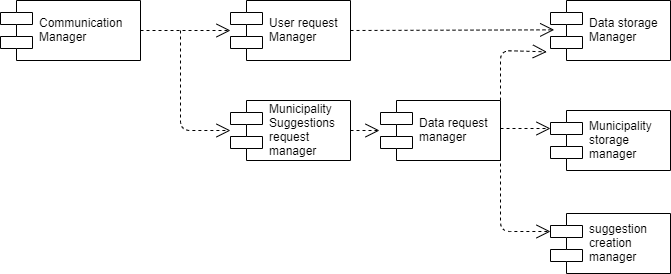
\includegraphics[scale=0.5]{Diagrams/Request application servers.png}
	\caption{Requests application server}
\end{figure}
\FloatBarrier

\textbf{Hierarchy of the modules of the reports application server\\}
\begin{figure}[h]
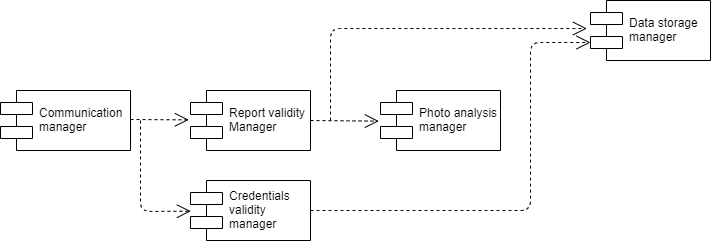
\includegraphics[scale=0.5]{Diagrams/report application server.png}
	\caption{Reports application server}
\end{figure}
\FloatBarrier


\begin{figure}[h]
\textbf{Hierarchy of the modules of the client smartphone application}
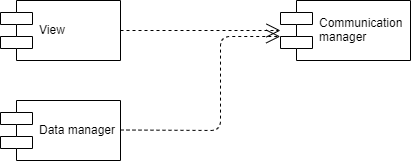
\includegraphics[scale=0.5]{Diagrams/Client.png}
	\caption{Client}
\end{figure}
\FloatBarrier

All the subsystems use the databases and so the databases (the system one and also the external one) will be the last components to be integrated into the subsystems. After the database is integrated, the subsystems will be tested again.\\

Up to know we have integrated all the components of the subsystems (The requests application server, the reports application server and the client) and so, in order to compose the entire system, we have to integrate and test all the subsystems together. For do that we have chosen a top-down approach as before. The first subsystem to be integrated will be the client, the second will be the servers (both the servers) and the last will be the databases. After every integration the result will be tested. After that all the subsystems will be integrated, the entire system will be formed.

\subsection{System testing}
The integrated system will have to be tested with black-box tests. This means that the code will be tested only from behavioural point of view and not structural. Functional and not functional requirements will be tested. The functional will be tested in order to test that the system meets the functional requirement. Instead, the non functional requirement can be about the performances, the load and the stress. All this aspects will have to be tested. To see what are the requirement (both functional of non functional) please, refer to the RASD to see them. 

\section{Effort spent}
\end{document}
